%================================================================
%                           N O T E S
%                           ---------
%
%                           ---------
%-----------------------------------------------------------------
%                       INTRODUCTION
%-----------------------------------------------------------------
\section{Introduction}
We now have an expression for the total field around the cyliner, the logical next step is to ask ourselves what happens \emph{inside} the cylinder. For this, we will assume that the boundary for the cylinder is permeable. Our goal in this section is to find an expression for the velocity field inside the cylinder, combine this with our result in Chapter \ref{chp:inside} to plot the complete field over the entire domain. \par
%
This is referred to as a \emph{transmission problem} in the literature, see for example \cite[$\S$1.3.3]{martin06scattering} since the wave is not bounded at the cylinder walls but transmitted through. We will consider a situation where the densities outside and inside the cylinder are different, see \figref{fig:problem_2}. \par
%
The statement of the problem is as follows. We are given an incident field, $\Phiin$ for which we need to find the field at the cylinder wall, $\Phi_{r=\sigma}$ and the field inside the cylinder wall $\Phi_{r<\sigma}$.
%
  \begin{figure} \centering
    %
    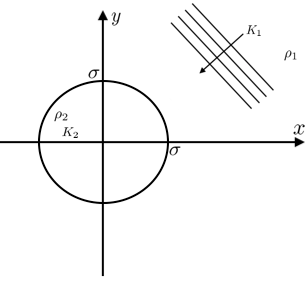
\includegraphics[width=6cm]{prob2/prob2_figures/prob2_sketch.png}
    %
    \caption{The transmission problem}\label{fig:problem_2}
    %
  \end{figure}
%
\section{The velocity field}
%
The velocity field inside the cylinder will be subject to the same physics as the one outside the cylinder. We can therefore find the scattered field inside the cylinder in the same way we found the scattered field outside the cylinder in section \ref{ss:scattered_field}. \par
%
In \ref{ss:scattered_field} we made our choice of cylindrical function to be used by describing the far field, and realising it must satisfy the Sommerfeld Radiation Condition (definition \ref{defn:sommerfeld_radiation_condition}). In the same way here we consider the field as we approach the origin.
%
\section{Problems at the origin}
%
  \begin{propn}
    Hankel functions are singular at zero.
  \end{propn}
  %
  \begin{proof}

  \end{proof}
%
  \begin{propn}
    Neumann functions are singular at zero.
  \end{propn}
  %
  \begin{proof}

  \end{proof}
%
  \begin{propn}
    Bessel functions are well defined at zero.
  \end{propn}
  %
  \begin{proof}

  \end{proof}
%
\section{The permeable boundary}
The first thing we notice when looking at this problem is the boundary condition: the wave must cross the permeable membrane of the cylinder to enter it, and this transition between the outside and inside must be continuous. We have:
%
  \begin{equation}\label{eq:in_boundary_conditon}
    \rho_1 \partialfrac{\Phi^{out}}{r}\bigg\vert_{r=\sigma} = \rho_2 \partialfrac{\Phi^{in}}{r}\bigg\vert_{r=\sigma}.
  \end{equation}\par
%
  \begin{propn}\label{propn:in_boundary_condition_integral}
    The boundary condition at $r=\sigma$ the velocity potential inside the cylinder is the following
    %
      \begin{align*}
        \Phi^{in}(r, \theta) = \sum^\infty_{n=0} \left( \xi_n r cos(n(\theta-\alpha)) + \vartheta_n(\theta) \right)& \\
        \text{ with } &\xi_n = \frac{\rho_1}{\rho_2}\epsilon_n i^n\{ B_n H_n'(k\sigma) + J_n'(k\sigma) \}
      \end{align*}
    %
    for $\vartheta_n$ any function of $\theta$.
  \end{propn}
%
  \begin{proof}
    This follows from \eqref{eq:in_boundary_conditon}. \par
    %
    We know that $\Phi^{out}$ is an infinite sum such that
    %
      \begin{gather*}
        \Phi^{out} = \sum^{\infty}_{n=0} \Phi^{out}_n, \text{ for } \\
        \Phi^{out}_n = \epsilon_n i^n cos(n(\theta-\alpha)) \{ B_n H_n(kr) + J_n(kr) \}.
      \end{gather*}
    %
    Then,
    %
      \begin{equation}
        \partialfrac{\Phi^{out}_n}{r}\bigg\vert_{r=\sigma} = \epsilon_n i^n cos(n(\theta-\alpha)) \{ B_n H_n'(k\sigma) + J_n'(k\sigma) \}.
      \end{equation}\par
    %
    Hence from \eqref{eq:in_boundary_conditon},
    %
      \begin{equation}
        \partialfrac{\Phi^{in}_n}{r} = \frac{\rho_1}{\rho_2}\epsilon_n i^n cos(n(\theta-\alpha)) \{ B_n H_n'(k\sigma) + J_n'(k\sigma) \},
      \end{equation}
    %
    or equivalently,
    %
      \begin{align}
        \partialfrac{\Phi^{in}}{r} &= \sum^\infty_{n=0} \xi_n cos(n(\theta-\alpha)). \\
        \therefore \Phi^{in} &= \bigintsss \sum^\infty_{n=0} \xi_n cos(n(\theta-\alpha)) \mathrm{d}r \\
          &= \sum^\infty_{n=0} \int\xi_n cos(n(\theta-\alpha)) \mathrm{d}r \\
          &= \sum^\infty_{n=0} \left( \xi_n r cos(n(\theta-\alpha)) + \vartheta_n(\theta) \right)
      \end{align}
    %
    as required.
  \end{proof}
%
